\par\Needspace{10\baselineskip}
\section{MAUDE duration exploration, paired comparison, and secondary diagnostic}
\label{supp:post-rc1}

\textbf{Status and scope.} C and D1 are new explorations on 28 prepared MAUDE snapshots covering 2019Q1--2025Q4, using the \texttt{DATE\_RECEIVED} clock. Validation and test periods had already been consulted in earlier development; these results therefore do not constitute independent confirmation. Counts concern only evaluated product--quarters with at least one positive link, at historical product support $\geq1$; they cover neither zero-positive observations nor a complete clinical population.

Provenance files comprise the manifests, preflights, epoch series, and metrics in \src{data/post_rc1}, as well as prepared snapshots under \src{data/real_R6/maude_B/prepared_snapshots.json.gz} (SHA-256 \src{1cba7f84ff24131715c68a985d9302c96c7bab4a4b2a27d906559a41104fbd36}). The runs use commits \src{4a22c2addc8203efd2b38a60c416270855c3bf3b} for C and \src{b14d878a78f559b65c70fc872a51a59af4c5ae85} for D1, the latter fixed before health-model training; code is provided under \src{vendor/post_rc1/healthgraphbench/tasks/maude/models.py}. The file \src{data/post_rc1/checkpoint_index.json} lists the nine included inference checkpoints: six C fits and three D1 none30 fits. Full candidate-score streams are not included.

\subsection{C: exploratory duration selection}

The validation fit uses history through 2022Q4 and evaluates 2023; scores under the protocol use the same 3,483 positive-containing product--quarters, 7,705 positive links, and 1,618,588 candidate pairs. Four independent fits without initialization from a preceding fit were compared, using the same dimension 8, eight sampled neighbors, learning rate 0.02, regularization 0.0005, BPR objective, $\tanh$ activation, and fixed negative-sampling and ranking rules. At zero epochs, no triplet is optimized; loss is not defined as an observed zero loss.

\begin{table}[!htbp]\centering\scriptsize
\caption{C: 2023 validation grid. BPR data loss is measured before updates and excludes regularization; no loss is observed at zero epochs. Fits are independent, and only the selected duration is evaluated on the C test periods.}
\label{tab:duration-rc2}
\begin{tabularx}{\linewidth}{@{}rXXr@{}}
\toprule
Epochs & Micro R@10 (hits / 7,705 positives) & BPR loss, epoch 1 $\rightarrow$ last & Triplet steps\\
\midrule
0 & 0.022193381 (171 / 7,705) & Not observed (no optimization) & 0\\
3 & 0.171576898 (1,322 / 7,705) & 0.692751769 $\rightarrow$ 0.315404017 & 203,028\\
10 & 0.166904607 (1,286 / 7,705) & 0.692751769 $\rightarrow$ 0.303309621 & 676,760\\
30 & 0.205061648 (1,580 / 7,705) & 0.692751769 $\rightarrow$ 0.210208402 & 2,030,280\\
\bottomrule
\end{tabularx}
\end{table}

The selection rule specified the maximum micro recall@10 across 3, 10, and 30 epochs, preferring the shortest duration in a tie. It selected 30 epochs on validation, and the lock was recorded at 17:32:26.207893 UTC before C's test evaluation. The zero-epoch fit is a descriptive reference, not an eligible duration for selection. The local lock attests to the reported ordering of files and runs; it does not undo prior exposure to the same periods.

Observed sensitivity is non-monotonic: ten epochs give lower validation recall than three, whereas thirty give the maximum on this grid. This does not mean that extending any training run improves its recall, or that thirty is an optimal duration.

\begin{figure}[!htbp]\centering
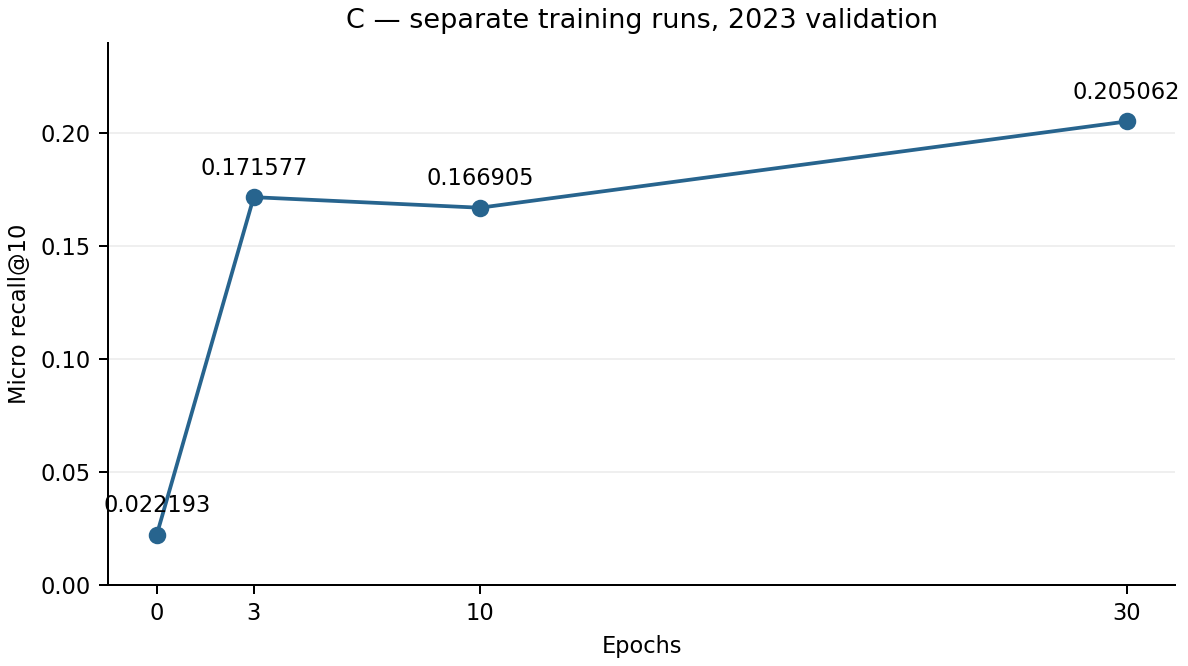
\includegraphics[width=\linewidth]{figures/maude_duration_RC2_en.png}
\caption{C: validation micro recall@10 by training duration. No training loss was observed for the zero-epoch fit.}
\label{fig:maude-duration-rc2}
\end{figure}

After selection, the chosen duration was fitted separately before 2024 and 2025, with rolling history between test quarters. On the 2024 test, micro recall@10 is $1,206/6,003=0.200899550225$; in 2025, $1,569/7,171=0.218797936132$. Summing hits and positive links across the two years gives $2,775/13,174=0.210642173979$, for 6,370 positive product--quarters and 2,975,156 candidate pairs. This pooled recall is not the arithmetic mean of the two annual recalls.

The historical benchmark test gave 0.172840443297 for three-epoch GraphSAGE and 0.192044936997 for neighbor frequency. These values remain unchanged. Prediction pairing, which is possible with retained historical outputs, must be distinguished from experimental control of duration. The absence of a new three-epoch fit in the C tests is not sufficient to make pairing impossible; conversely, matching keys and denominators do not demonstrate that duration alone explains a difference between training runs.

\subsection{Comparing the historical path with the C calculation}

The historical individual file records execution commit \src{ca0d64b2738c3f36637196cfb14d2fe4115a7c37}; \src{b010d5a49eae56837a920b2e30dece41c42c0c44} identifies the cited benchmark source state. Their role is distinct from C commit \src{4a22c2addc8203efd2b38a60c416270855c3bf3b}. Comparing sources between the historical execution and C shows no change to \src{evaluate.py}. In \src{models.py}, C adds loss/state callbacks and checkpoint reconstruction, and extracts the final representation calculation into a function.

\begin{table}[!htbp]\centering\footnotesize
\caption{Historical--C comparison of the mean-aggregation path. It describes code and retained evidence, not a new historical execution on health data.}
\begin{tabularx}{\linewidth}{@{}p{34mm}X@{}}
\toprule
Element & Comparison finding\\
\midrule
Initialization and neighborhood & Sorted node orders, sinusoidal vectors with salts 11/17, initial identity/0.25 transformations, and deterministic sampling of eight neighbors are unchanged.\\
Triplets and optimization & Product/positive order, epoch-dependent hashing, exclusion of positive neighbors, BPR coefficient, gradients, and regularized updates are unchanged; C adds counters and pre-update loss.\\
Representation and score & Same one-hop mean, $\tanh$, dot product, and zero fallback; extraction of the final calculation and raw-state export, without changing these operations.\\
Evaluation & Evaluation source unchanged; the new runner reads prepared snapshots, fits at annual origins, holds representations fixed during the year, and updates history after each quarter.\\
Evidence and limit & Retained preflight: 364 identical three-epoch scores on three non-empty fixtures, plus an empty case and checkpoint reconstruction. This non-health check does not prove equivalence of all possible executions.\\
\bottomrule
\end{tabularx}
\end{table}

Preflight reports and their fingerprints remain in \src{data/post_rc1/C_preflight.json}. Prepared snapshots do not expose every field of the historical \src{DataBundle}; this comparison concerns the graph-based GraphSAGE path, not all tabular methods. No historical model is retrained for this source verification. It supports interpreting C as configuration sensitivity, without turning selection on previously examined periods into a confirmatory experiment or a general causal effect of duration.

\subsection{GraphSAGE30--neighbors: paired comparison and conditional CI}

After this additional analysis was authorized on 3 October 2026, the protocol was fixed before the new calculation: 2024Q1--2025Q4 test, micro recall at ten, GraphSAGE30-minus-neighbors difference, 1,000 product draws with replacement, and seed 20261003. The selected model and historical results were already known; this calculation lock is therefore neither an external preregistration nor a correction for selection. No model is trained or scored.

Keys (product, quarter), support, and positive-problem sets agree across 6,370 observations, 13,174 positive links, and 2,026 products. C's complete candidate lists are checked against lists reconstructed from prepared snapshots and the unchanged historical rule; they total 2,975,156 pairs. The historical export does not retain its complete lists: it provides cardinalities and sampled positive/non-positive predictions. Agreement of reconstructed lists with C and of cardinalities/positives with the historical export is therefore established, not byte-for-byte identity of two complete exports. Any discrepancy would have stopped the analysis; no observation is removed through an opportunistic intersection.

Historical hits are read from \src{entity_metrics}, and C hits from retained ranks/labels, without recalculating scores. GraphSAGE30 retrieves 2,775 links and neighbors 2,530, on the same denominator of 13,174. The difference is $+0.018597236982$ and the conditional 95\,\% CI is $[+0.011975077183;+0.025570110820]$. Each draw keeps every quarter of a product together and recalculates the ratio of sums; this is neither a mean of product recalls nor independent resampling of quarters. The 2.5 and 97.5\,\% quantiles use linear interpolation; all 1,000 draws are defined.

The interval is conditional on the observed predictions and population. It covers neither validation selection, training variability, all network dependence between products, nor transfer to another population. It is neither independent confirmation nor a causal duration effect. It applies neither to historical three-epoch GraphSAGE nor to D1.

Pinned inputs, the protocol, contribution CSV, and draws are under \src{data/post_rc1/paired_*}; the source comparison is described in \src{verification/rc2_paired/code_bridge.json}. The completed calculation takes 7.969 s, with peak RSS of 488,841,216 bytes, below the 900 s / 512 MiB ceilings. A first attempt stopped before the draws: an address-space limit had been confused with the RSS ceiling. This mistakenly added restriction was removed without changing the RSS/time/output ceilings or statistical protocol; the record is retained in \src{verification/rc2_paired/attempt_1_failure.json}.

\paragraph{Original calculation in the repository, with retained outputs.}
\begin{Verbatim}[fontsize=\footnotesize]
python scripts/analyze_maude_paired_comparison.py \
  --protocol results/maude_paired_protocol_20261003.json \
  --output-dir NEW/maude_paired
\end{Verbatim}

\paragraph{Compact replay from the package root, without original inputs.}
\begin{Verbatim}[fontsize=\footnotesize]
PYTHONPATH=vendor/post_rc1 python \
  scripts/analyze_maude_paired_comparison.py \
  --protocol data/post_rc1/paired_protocol.json \
  --replay-contributions data/post_rc1/paired_contributions.csv \
  --output-dir NEW/maude_paired_replay
\end{Verbatim}
Use a new destination and an environment with NumPy (original calculation: Python 3.13.5, NumPy 2.3.5). Compact replay reproduces the contrast and draws but does not recheck original candidate identities. C/D1 checkpoints are included separately; their earlier audits are not rerun for this CI.


\subsection{D1: secondary neighborhood-removal diagnostic under fixed settings}

D1 compares C's 30-epoch \emph{mean} model, reused without refitting, with one new 30-epoch \emph{none} model. The shared duration comes from C and the fixed D1 protocol; no duration grid or duration tuning was conducted in D1. The same periods and evaluation rules are used for both variants: candidate identifiers, labels, support counts, hashed negatives, and ranking conventions agree. Both models retain trainable node-identity vectors. The \emph{none} model computes $h=\tanh(W_{\mathrm{self}}x)$ from the node's own vector only; it does not aggregate neighbors and is not a GNN.

Absence of message passing does not mean absence of relational information: \emph{none}'s identity vectors are learned from the same historical edges and BPR. D1 compares two ways of calculating and learning representations. Duration was selected for \emph{mean}, then imposed on \emph{none}; no control-specific tuning established its ability to optimize this task effectively.

The \emph{mean} variant has 128 active shared-transformation scalars, compared with 64 for \emph{none}; the number of node-vector scalars is the same in each pair of fits. This 64-parameter difference must be declared, but it does not demonstrate that capacity explains the gap. The imposed duration and the control's nearly flat loss are also essential to interpreting this diagnostic. The contrast does not isolate a causal aggregation effect at equal capacity.

D1 was locked at 20:53:30.842192 UTC using validation, before its first D1-specific tests. However, the C test results for \emph{mean} were already available at that lock, and the test periods had been consulted earlier. Thus, the ordering of the D1 lock and its tests does not make this an independent confirmation.

\begin{table}[!htbp]\centering\scriptsize\setlength{\tabcolsep}{2.5pt}
\caption{D1: micro recall@10 on cohorts with at least one positive link, at historical support $\geq1$. Mean30 is retained from C; none30 was newly fitted in D1. Hits are shown in parentheses. No interval is attached to the contrast.}
\label{tab:aggregation-rc2}
\begin{tabularx}{\linewidth}{@{}XrXXr@{}}
\toprule
Cohort & Positive links & Mean30 R@10 (hits) & None30 R@10 (hits) & Mean $-$ none\\
\midrule
Validation 2023 & 7,705 & 0.205061648 (1,580) & 0.031148605 (240) & $+0.173913043$\\
Test 2024 & 6,003 & 0.200899550 (1,206) & 0.036481759 (219) & $+0.164417791$\\
Test 2025 & 7,171 & 0.218797936 (1,569) & 0.034862641 (250) & $+0.183935295$\\
Pooled test 2024--2025 & 13,174 & 0.210642174 (2,775) & 0.035600425 (469) & $+0.175041749$\\
\bottomrule
\end{tabularx}
\end{table}

On the pooled test, mean30 obtains $2,775/13,174=0.210642173979$ and none30 $469/13,174=0.035600425080$; the signed descriptive mean30--none30 difference is $+0.175041748899$. No confidence interval or statistical test is attached to this difference. The figure also shows the annual contrasts and recorded losses.

\begin{figure}[!htbp]\centering
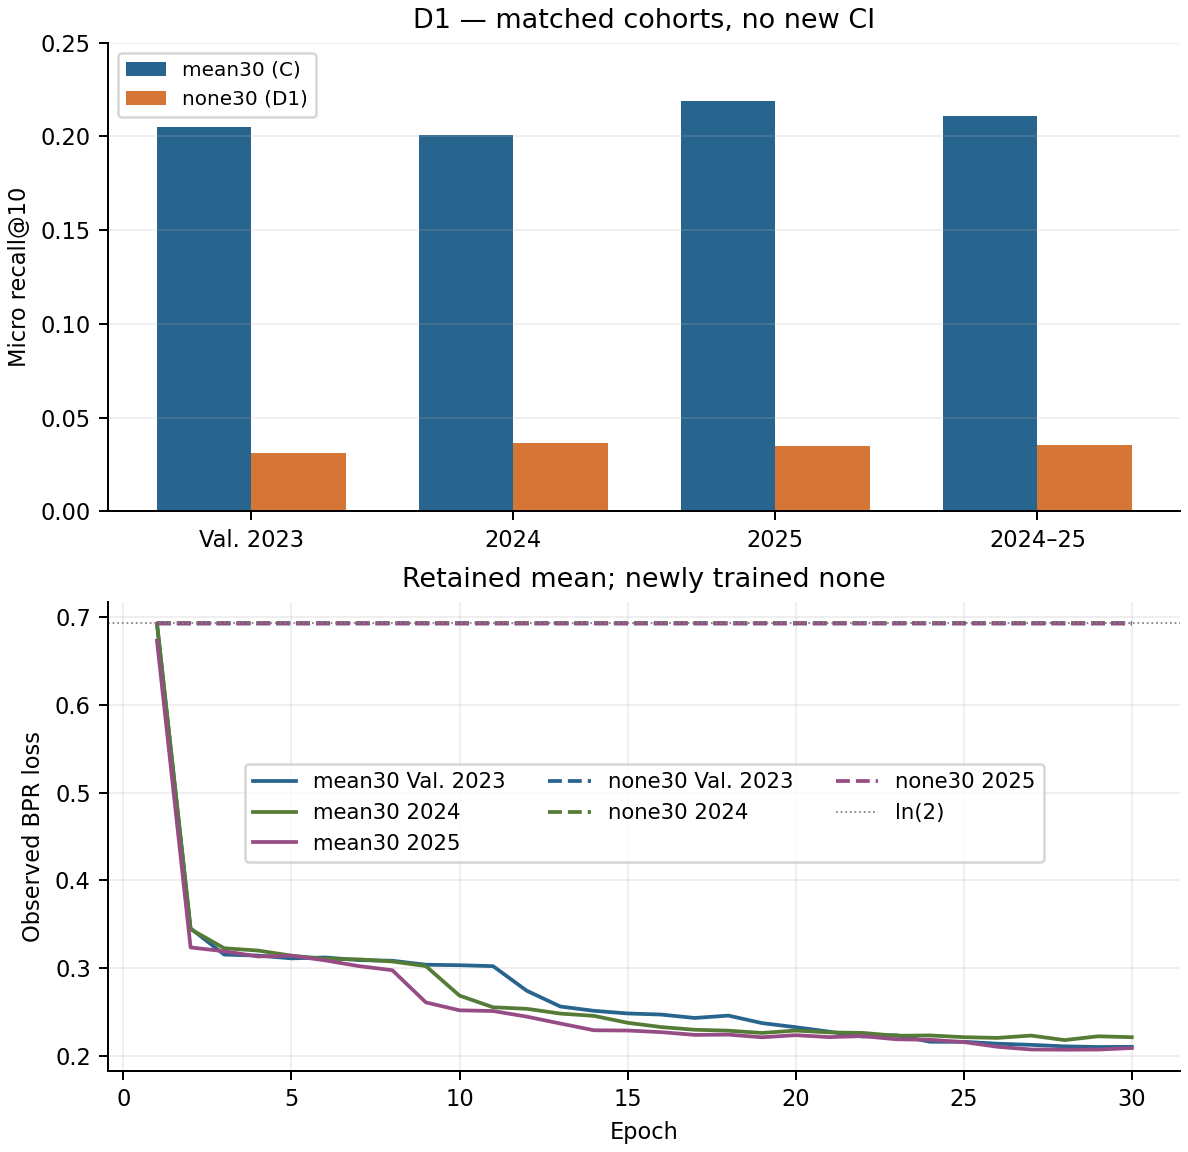
\includegraphics[width=\linewidth]{figures/maude_aggregation_RC2_en.png}
\caption{D1: micro recalls@10 in the upper panel; observed losses in the lower panel. Mean30 is reused from C; only the none30 fits are new in D1. Pooled recall combines the two test years and is not an additional distinct cohort.}
\label{fig:maude-aggregation-rc2}
\end{figure}

The three none30 fits comprise 90 observed epochs, 6,756,720 steps, and no skipped positives. The exported data loss, the pre-update mean of $\operatorname{softplus}(-\text{margin})$ excluding regularization, remains close to $\ln(2)$ with no observed decrease (about 0.693132--0.693145 at the first epoch and 0.693147 at the thirtieth). This finding is more informative about the control's scope than recall-bar height alone: it does not establish effective learning under the retained parameters. However, it identifies neither a bug, representation collapse, too few epochs, nor another cause of failure. D1 remains a sensitivity diagnostic for neighborhood removal under fixed settings, not a demonstration of the causal benefit of aggregation.

\subsection{Audits, costs, and scope of verification}

C and D1 audits concern the new fits and do not replace the historical B1/B2 reconstruction in S10. The C audit reconstructs scores from six raw checkpoints and checks 9,449,508 predictions, 24 fit-quarters, and 20,302 candidate lists; no discrepancy is detected, with an absolute tolerance of $10^{-12}$ for floating-point values. The report is retained under \src{verification/post_rc1/C_numeric_audit.json}, with the manifest \src{data/post_rc1/C_manifest.json}. The earlier B1/B2 reconstructions recovered training inputs and node inventories without inspecting historical checkpoints.

The D1 audit reconstructs none30 scores from three raw checkpoints and pairs them with C's retained mean30 outputs. It checks 4,593,744 new scores, 9,853 candidate lists per variant, 12 quarters, and 51,260,776 numerical checks; no discrepancy is detected at the absolute tolerance of $10^{-12}$. The 9,187,488 candidate identifiers are the sum of the two exports, or 4,593,744 pairs on each side. The D1 audit took 58.547 s. Its final memory readings diverge: $118,292,480$ bytes for \texttt{VmHWM} and \texttt{VmRSS}, versus $571,580,416$ bytes for \texttt{ru\_maxrss}. In the absence of startup readings, it is not possible to certify that the entire audit stayed below 512 MiB or to attribute the discrepancy with certainty to the process or launcher. An independent telemetry probe shows that a different scope after \texttt{exec} can explain the discrepancy, without establishing the exact source of this audit measurement. Both values remain recorded in \src{data/post_rc1/post_rc1_metrics.json}.

For training phases, the limits were 900 s, 512 MiB aggregate RSS, and 512 MiB of output per phase, with one worker and a single-threaded environment; each reported C and D1 phase finished within these limits, without retries. C totaled 1,167.908 s across its phases (maximum aggregate RSS peak 249,405,440 bytes); this sum across multiple phases was not subject to a global 900-s limit. D1 totaled 416.144 s (maximum aggregate RSS peak 303,284,224 bytes). Mean30 measurements are from C and were reused; they are not new fitting costs incurred by D1. These costs do not establish equal CPU budgets between variants or runs.

These checks establish numerical consistency of RC2 outputs with the prepared snapshots, checkpoints, and audited logs. They do not verify historical public availability of every field, undo prior exposure to the periods, provide independent confirmation or clinical benefit, or justify causal or general claims about graphs.